\begin{document}
		% La versió relaxada del problema i la seva solució en Index de Gittins i Upper confidence bound
	\subsection{Upper confidence bound}
	Que el problema es mostri com a PSPACE-hard significa que el càlcul del mínim és, si no es demostra la igualtat entre
	les diferents complexitats, tan dificultós que deixa de ser pràctic intentar-ho. Per sort, el problema relaxat a un
	\textit{k-armed bandits} dona una bona heurística al problema principal. Aquest ja hem dit que és decidible amb una complexitat P
	 per l'índex de Gittins, però el problema recau en el cost de calcular aquest índex, ja que tot i que sigui polinomial en el temps
	el cost és bastant elevat, pel que s'utilitzen altres algoritmes que tot i no ser perfectes es queden molt propers a l'òptim del 
	problema relaxat. Amb aquests algorismes trobem el d'\textit{Upper confidence bound}. \\
	\\
	L'algorisme UCB fa les seleccions de a quina màquina jugar en base a l'optimisme. Es a dir, centrant-nos en el millor que pot acabar sent una acció.
	Seguint aquesta estrategia, per exemple una heurística possible és fer la selecció de la màquina seguint la seguent formula:\\\\ %TODO ficar formula
	On Qn(a) és el valor actual d'una màquina escura-butxaques a. El valor sota l'arrel és el logartime del nombre de màquines a les que hem jugat dividit per kn, que és el nombre de tirades que hem fet en la màquina a. I finalment c és una constant.\\
	Per tal de calcular Qn(a) podem fer una mitjana:\\\\ %TODO ficar formula
	On Rn és la recompensa que obtenim de realitzar aquesta acció.\\\\
	\begin{lstlisting}[language=Python]
import numpy as np 
import matplotlib.pyplot as plt 
import pandas as pd
class ucb_bandit:
    '''
    Upper Confidence Bound Bandit
    
    Inputs 
    ============================================
    k: number of arms (int)
    c:
    iters: number of steps (int)
    mu: set the average rewards for each of the k-arms.
        Set to "random" for the rewards to be selected from
        a normal distribution with mean = 0. 
        Set to "sequence" for the means to be ordered from 
        0 to k-1.
        Pass a list or array of length = k for user-defined
        values.
    '''
    def __init__(self, k, c, iters, mu='random'):
        # Number of arms
        self.k = k
        # Exploration parameter
        self.c = c
        # Number of iterations
        self.iters = iters
        # Step count
        self.n = 1
        # Step count for each arm
        self.k_n = np.ones(k)
        # Total mean reward
        self.mean_reward = 0
        self.reward = np.zeros(iters)
        # Mean reward for each arm
        self.k_reward = np.zeros(k)
        
        if type(mu) == list or type(mu).__module__ == np.__name__:
            # User-defined averages            
            self.mu = np.array(mu)
        elif mu == 'random':
            # Draw means from probability distribution
            self.mu = np.random.normal(0, 1, k)
        elif mu == 'sequence':
            # Increase the mean for each arm by one
            self.mu = np.linspace(0, k-1, k)
        
    def pull(self):
        # Select action according to UCB Criteria
        a = np.argmax(self.k_reward + self.c * np.sqrt(
                (np.log(self.n)) / self.k_n))
            
        reward = np.random.normal(self.mu[a], 1)
        
        # Update counts
        self.n += 1
        self.k_n[a] += 1
        
        # Update total
        self.mean_reward = self.mean_reward + (
            reward - self.mean_reward) / self.n
        
        # Update results for a_k
        self.k_reward[a] = self.k_reward[a] + (
            reward - self.k_reward[a]) / self.k_n[a]
        
    def run(self):
        for i in range(self.iters):
            self.pull()
            self.reward[i] = self.mean_reward
            
    def reset(self, mu=None):
        # Resets results while keeping settings
        self.n = 1
        self.k_n = np.ones(self.k)
        self.mean_reward = 0
        self.reward = np.zeros(iters)
        self.k_reward = np.zeros(self.k)
        if mu == 'random':
            self.mu = np.random.normal(0, 1, self.k)
	
	\end{lstlisting}
Aquesta és la classe en la qual definim el problema. Per tal utilitzar-la i obtenir-ne resultats, podem executar el seguent còdi:
	\begin{lstlisting}[language=Python]
	
k = 10 # number of arms
iters = 1000
ucb_rewards = np.zeros(iters)
# Initialize bandits
ucb = ucb_bandit(k, 2, iters)
episodes = 1000
# Run experiments
for i in range(episodes): 
    ucb.reset('random')
    # Run experiments
    ucb.run()
    
    # Update long-term averages
    ucb_rewards = ucb_rewards + (
        ucb.reward - ucb_rewards) / (i + 1)
    
plt.figure(figsize=(12,8))
plt.plot(ucb_rewards, label="UCB")
plt.legend(bbox_to_anchor=(1.2, 0.5))
plt.xlabel("Iterations")
plt.ylabel("Average Reward")
plt.title("Average UCB Rewards after " 
          + str(episodes) + " Episodes")
plt.show()
	
	\end{lstlisting}
	  
Aquest còdi ens farà un plot en el qual podem veure l'evolució de l'agent:\\

\begin{figure}[h!]
 \centering
  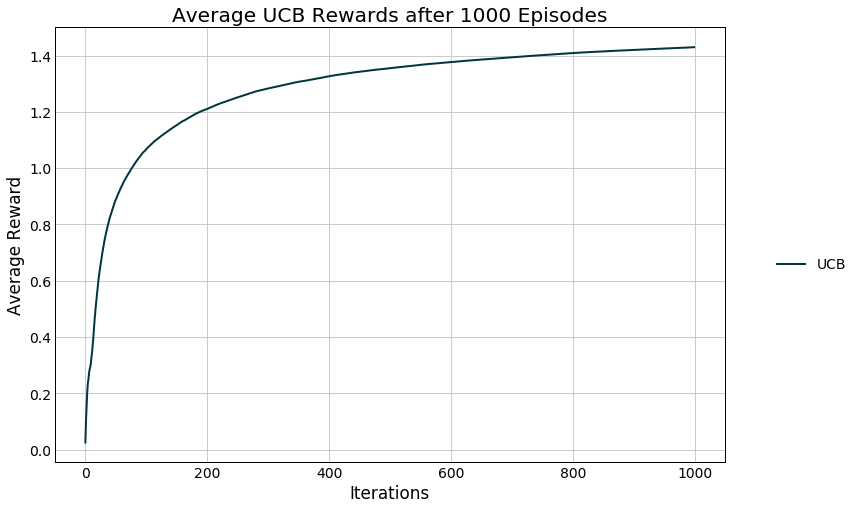
\includegraphics[width=0.9\textwidth]{results.png}
 \caption{Result plot simulation multi-armed bandit}
 \end{figure}
	  
\end{document}